% Scalar instruction entry source: tools/generate_scalar_instruction_catalog.py.
\subsection{\texttt{MADD}}
\label{sec:scalar-madd}
\index{MADD@\texttt{MADD}}
\begin{sloppypar}\noindent\textbf{Purpose.} Multiply-add (three-source).\end{sloppypar}\smallskip
\noindent\textbf{Syntax.}\par
\begin{lstlisting}[style=ptoscalarcode]
madd SrcL, SrcR, SrcD, ->RegDst
\end{lstlisting}
\noindent\textbf{Encoding.}\par
\noindent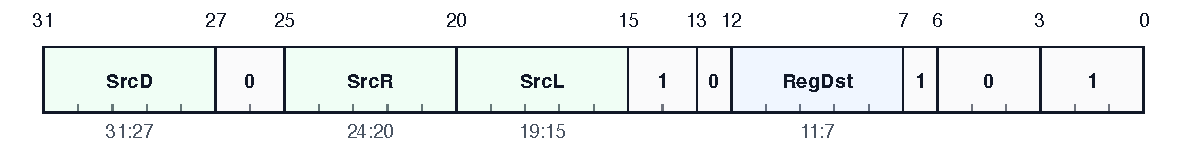
\includegraphics[width=\textwidth]{figs/encoding/scalar_instruction_entries/enc_madd.pdf}\par\smallskip
\begin{description}[leftmargin=0.18\linewidth,style=nextline]
\item[Format] \texttt{L32} \texttt{32-bit} scalar word.
\item[Pattern] \texttt{.....00..........110.....1000111}.
\end{description}
\noindent\textbf{Classification.}\par
\begin{description}[leftmargin=0.18\linewidth,style=nextline]
\item[Category] Integer ALU and Bit-Manipulation.
\item[Family] Multi-Cycle ALU.
\item[Execution class] \texttt{ALU}; uop\_kind=ALU, alu\_kind=ALU\_MULTI\_CYCLE.
\end{description}
\noindent\textbf{Operand fields.}\par
\begin{description}[leftmargin=0.18\linewidth,style=nextline]
\item[\texttt{RegDst}] Bits \texttt{11:7 (5b)}. 5-bit scalar destination register written by this instruction; X0 is hardwired to zero, so writes to X0 are ignored.
\item[\texttt{SrcD}] Bits \texttt{31:27 (5b)}. 5-bit scalar source register containing the data operand consumed by the instruction.
\item[\texttt{SrcL}] Bits \texttt{19:15 (5b)}. 5-bit scalar source register used as the left input operand.
\item[\texttt{SrcR}] Bits \texttt{24:20 (5b)}. 5-bit scalar source register used as the right input operand before any encoded modifier or shift is applied.
\end{description}
\noindent\textbf{Operation.}\par
\begin{lstlisting}[style=ptoscalarcode]
a = Read(SrcL)
b = Read(SrcR)
d = Read(SrcD)
result = LowProduct(a, b) + d
Write(RegDst, result)
\end{lstlisting}
\Needspace{0.08\textheight}
